%!TEX root = ../thesis.tex

\chapter{Combined Schottky + Isochronous Mass Spectrometry (\textsc{S+IMS})}\label{chap:chap2:methodology}
\lettrine{H}{erein}, I present the foundations of a novel methodology for investigating the nuclear two-photon decay at storage rings and other high-precision mass and half-life measurements by combining the isochronous mode of a storage ring with non-destructive resonant Schottky cavities hence \textsc{S+IMS}. Specially, we focus on the Experimental Storage Ring~(\textsc{ESR}) at the heavy-ion research facility \textsc{GSI}. The techniques and approaches described herein are crucial for the advancement of storage ring mass spectrometry.
\newpar 
An overview of the experimental setup employed is presented in \cref{sec:chap2:experimentalsetup}, which is subdivided into production (\cref{subsec:chap2:production}), storage (\cref{subsec:chap2:storage}), and detection (\cref{subsec:chap2:detection}). 
\Cref{sec:chap2:isomode} discusses the isochronous mode of the ring, detailing how it can be quantified and monitored in real time (in-line) using the electron cooler, as discussed in \cref{subsec:chap2:ecoolercurve}, and through off-line analysis, as outlined in \cref{subsec:chap2:isocurve}.
In~\cref{sec:chap2:datamanipulation}, we detail the steps followed during the data analysis, encompassing data classification (\cref{subsec:chap2:dataclassification}), Schottky-based ion identification (\cref{subsec:chap2:identification}), mass determination (\cref{subsec:chap2:massdetermination}), and half-life determination~(\cref{subsec:chap2:halflifedetermination}).

\section{Experimental setup}\label{sec:chap2:experimentalsetup}
The Gesellschaft für Schwerionenforschung~\cite{GSI} (\textsc{GSI}) facility is a forefront center for research in atomic and nuclear physics located in Darmstadt, Germany. It specializes in the production and acceleration of heavy ions for various scientific experiments, from fundamental physics research~\cite{Loetzsch2024} to applications in material science~\cite{matscience} and medicine~\cite{kraft2013history}. Here took place the realization of experiment \textsc{E143}~\cite{kortenE143}, where the isolated nuclear two-photon decay was measured for the first time. Therefore, the whole setup and its functions during the different stages: production  (\cref{subsec:chap2:production}), storage (\cref{subsec:chap2:storage}), and detection (\cref{subsec:chap2:detection}), will be elucidated.
\begin{figure}[hbt]
    \includegraphics[width=\textwidth]{gsi_facility.png}
    \caption{\textsc{GSI} accelerator facility. Details of the facility will be discussed in the text. Based on \cite{GSIWebsite}.}
    \label{fig:chap2:gsi}
\end{figure}
\newpar
\Cref{fig:chap2:gsi} shows a scheme of the accelerator facility at \textsc{GSI}. This facility has the capability to produce and accelerate highly-charged ions from hydrogen up
to uranium (see \cref{subsec:chap2:production}). The ion source is the starting point for the production of positively charged ions (\cref{subsubsec:chap2:sources}). The produced lowly-charged ions (of a single species) are then accelerated in different stages by linear and circular accelerators (\cref{subsubsec:chap2:accelerators}). When the ions have reached relativistic energies, they are impinged on solid Be targets of a determined thickness in order to produce the desired fragments via projectile fragmentation (\cref{subsubsec:chap2:fragmentation}). Depending on the needs, independent nuclei species can be separated (purified) by the FRagment Separator~\cite{FRS} (\textsc{FRS}) or all the fragments can be directly inserted into the experimental storage ring (\textsc{ESR}) through the \textsc{TE-line}. Once stored within the \textsc{ESR} (\cref{subsec:chap2:storage}), we can perform a variety of experiments with the different elements and detectors (\cref{subsec:chap2:detection}). If needed, the produced fragments can be decelerated and transferred to a lower-energy ring, the \textsc{CRYRING}~\cite{cryring,cryringGSI}, or to the ion-trap facility \textsc{HITRAP}~\cite{hitrap}.

\subsection{Production}\label{subsec:chap2:production}
\subsubsection{Initial stages}\label{subsubsec:chap2:sources}
The initial stage of ion production involves the creation of high-current ion beams. Two primary mechanisms facilitate ion generation: photoionization~\cite{Photoionization}, where ions are produced through photon collisions, and impact ionization~\cite{impactionization}, resulting from electron collisions. Depending on the mechanism and materials involved, there are several types of ion sources~\cite{ionsourcesGSI}:

\begin{itemize}
    \item \textbf{Filament driven ion sources:} These include the Multi Cusp Ion Source (\textsc{MUCIS}) and its advanced versions, as well as \textsc{CHORDIS} (Cold or Hot Reflex Discharge Ion Source), which are essential for creating dense plasma environments to facilitate ion production. Notably, \textsc{MUCIS} has been extensively studied and applied in various applications, including cyclotrons, due to its ability to confine ions effectively within cusp geometries of magnetic fields, thus enhancing beam currents.
    \item \textbf{Vacuum arc driven ion sources:} Including the Metal Vapor Vacuum Arc Ion Source (\textsc{MEVVA}) and \textsc{VARIS} (Vacuum Arc Ions Source). They employ metal vapors to generate ion beams. These sources make use of a vacuum arc mechanism to ionize metal vapors, which is crucial for applications requiring heavy metal ions.
    \item \textbf{High duty factor sources:} Such as the \textsc{PIG} (Penning Ionization Gauge).
    \item \textbf{Electron cyclotron resonance (ECR) sources:} \textsc{ECRIS} (Electron Cyclotron Resonance Ion Source), uses microwave technology to ionize gases in a magnetic field. This was the one employed for producing initially the ions of \,\isotope{78}{Kr}.
\end{itemize}

\subsubsection{Acceleration}\label{subsubsec:chap2:accelerators}
The acceleration of ions is a critical step in preparing them for experiments. At \textsc{GSI} we have a combination of linear and circular accelerators. While linear accelerators are dominated by radiofrequency cavities, the circular ones primarily utilize magnets \cite{Conte}.
\newpar
As the first acceleration stage, the \textsc{GSI} facility uses the \textsc{UNILAC} (UNIversal Linear ACcelerator), which is composed of three parts:
\begin{itemize}
    \item \textbf{\textsc{UNILAC} Wideroe accelerator:} Operates at a frequency of $27$\,MHz, accelerating ions from zero to $2\cdot10^{6}$\,km/h. For that it employs a voltage range of $20$\,kV to $130$\,kV. Within it, the ions reach speeds of $\beta \approx 0.2$\,\%.
    \item \textbf{Connection line to the Alvarez accelerator:} Composed of several single-cavity resonators and a gas-stripper for enhancing the acceleration efficiency, reaching $\beta \approx 6$\,\%.
    \item \textbf{\textsc{UNILAC} Alvarez accelerator:} Following the Wideroe accelerator, this accelerator operates at a higher frequency of $108$\,MHz. It uses a standing wave to accelerate ions to $\beta \approx 16$\,\%, or equivalently to energies of $11.4$\,MeV/u.
\end{itemize}

Once ions have received this initial acceleration, they are transferred to the synchrotron \textsc{SIS-$18$} through a process involving a foil stripper and charge state separation. 
\newpar
The \textsc{GSI} synchrotron \textsc{SIS-$18$}, known as \textsc{SchwerIonenSynchrotron}, is a key component of the \textsc{GSI} facility, designed for the acceleration of a wide range of ions, from protons ($4$\,GeV, $\beta \approx 98$\%) to highly-charged uranium ions ($1$\,GeV/u, $\beta \approx 88$\%). This can be achieved due to its characteristics; it has a circumference of $216$\,m, a bending radius of $10$\,m and a maximum magnetic field strength of $18$\,T, along with RF cavities working from $0.85$\,MHz to $6$\,MHz, and an ultra-high vacuum of $10^{-11}$\,mbar. 

\subsubsection{Projectile fragmentation}\label{subsubsec:chap2:fragmentation}
At relativistic velocities, nuclear collisions are extremely violent, and a vast range of fragments can be created~\cite{projectilefragmentation}. The reaction is not selective in terms of its products, but the forward momentum of each fragment allows for precise identification using time-of-flight and energy-loss techniques to determine their mass and charge. 
The efficiency of fragment production is constrained by the thickness of the target, which is chosen to minimize energy and angular straggling at maximum fragment production. 
Once created, the fragments can be filtered via the FRagment Separator or can be injected directly into the \textsc{ESR} through a direct beam line, the \textsc{TE-line}.
\newpar
The FRagment Separator\footnote{Please note that the \textsc{FRS} was not used in this experiment; however, it is included here to provide a complete overview for the thesis.} \cite{FRS} (\textsc{FRS}) is configured by a set of two dipoles, a degrader, and two more dipoles designed for implementing the $B\rho-\Delta E-B\rho$ separation technique. Time-of-flight (\textsc{ToF}) measurements are employed between the $\Delta E-B\rho$ section for particle identification, complemented by the use of time projection chamber (\textsc{TPC}) detectors for spatial positioning measurements, and plastic scintillators for \textsc{ToF}. This method enables the filtration of fragments, allowing for the selection of specific species, as demonstrated in \cite{Dellmann2024}.
\newpar
The \textsc{TE-line} serves as the direct transfer line between the \textsc{SIS}-$18$ and the \textsc{ESR}, facilitating the transfer of all produced fragments into the \textsc{ESR}, which operates as a mass spectrometer. Utilizing slits, as described in \cref{subsubsec:chap2:brocut}, enables the exclusion of undesired ions (contaminants). Due to the high demand for \textsc{FRS} usage, experiments that can be executed through the \textsc{TE-line} receive priority in beam time scheduling, as was the case with the \textsc{E143} experiment \cite{kortenE143}. Additionally, the direct line enables faster extraction compared to the FRS, with a time of approximately $500\,\mu$s.
\newpar
Via using \textsc{LISE++}~\cite{lise++}, we are able to simulate both the reaction leading to the creation of fragments and their subsequent transmission to the storage ring. It enables the prediction of fragment production rates, ion optical settings for optimal fragment selection, and the efficiency of transmission through simulated beam lines to the storage ring. Thus, the fragments predicted by \textsc{LISE++} serve as a first (realistic) estimate for what we should encounter in the ring during identification (more in \cref{subsubsec:chap2:rionid}). 
\subsubsection{\textsc{$B\rho$-cut}}\label{subsubsec:chap2:brocut}
By using the \textsc{TE-line}, the only way to filtrate the fragments is by utilizing mechanical slits. With them, we are able to select a specific $B\rho$ range (window). By placing these slits at different planes and positions, it is possible to manually exclude particles on certain orbits without affecting the selected $B\rho$ range, hence performing a \textsc{$B\rho$-cut}. This approach somewhat reduces the number of contaminants and narrows the allowed momentum spread to a more uniform area, particularly regarding $\gamma_t$. The relative momentum spread before entering the \textsc{ESR} exceeds $1$\,\%, but after the $B\rho$-cut, it can be reduced to approximately $0.01$\,\%.
\newpar
As a result of this selection process, the distribution of particles in terms of their $B\rho$ values becomes non-symmetric (as depicted in \cref{fig:chap2:brhocut}), being one of the reasons to the observed deformation in the peak shape. This produces the selection of more particles at either higher or lower $B\rho$ values compared to the mean 
\begin{figure}[hbt]
    \centering
    \includegraphics[width=0.75\textwidth]{brho_cutted.png}
    \caption{Illustration of the \textsc{$B\rho$-cut} over some expected yields of fragments by \textsc{LISE++}.}
    \label{fig:chap2:brhocut}
\end{figure}

\subsection{Storage}\label{subsec:chap2:storage}
The ions are transferred to and confined into the experimental storage ring~\cite{ESR}. Since recently \textsc{GSI} counts with another storage ring with smaller dimensions~\cite{cryring, cryringGSI}, designed for lower energies.
This experiment utilized only the \textsc{ESR}, in which we will focus on in greater detail. Storage rings share the same principles as circular accelerators but tailored for specific research applications, as was introduced already in \cref{subsec:intro:storage_ring_mass_spectro}. Like in circular accelerator, its capabilities are defined mostly by their geometry and dipole magnet strength, i.e. they are governed by \cref{eq:intro:brho}.
\newpar
\begin{figure}[hbt]
    \centering
    \includegraphics[width=0.75\textwidth]{esr300dpi.png}
    \caption{The experimental storage ring (\textsc{ESR}) and its main characteristics. For details see text.}
    \label{fig:chap2:esr}
\end{figure}
As shown in \cref{fig:chap2:esr}, the \textsc{ESR} has a circumference of $108$\,meters (half of the \textsc{SIS}-$18$) and is composed of six $60^\circ$ dipole magnets, with a maximum magnetic rigidity of up to $10$\,Tm. This allows the storage ring to operate over a broad energy range from $4$\,MeV/u to $420$\,MeV/u, therefore the revolution frequency of the ions revolving the storage ring ranges approximately between $0.6$\,MHz to $2$\,MHz. In addition, it maintains an ultra-high vacuum of $2\times10^{-11}$\,mbar to significantly reduce interactions with residual gases, and multiple mechanism for cooling (see \cref{subsec:intro:cooling}). All of this enables high-precision studies on masses, half-lives and nuclear reactions for atomic, nuclear and astrophysics motivations. In \cref{fig:chap2:esr} are shown the locations of the detectors used during the \textsc{E143}, the $245$\,MHz~\cite{Sanjari_2013} and $410$\,MHz~\cite{Sanjari-410} resonant Schottky cavities. More details are given in \cref{subsec:chap2:detection}.

\subsection{Detection}\label{subsec:chap2:detection}
%Schottky cavities + scalars + RSAs + NTCAP (signal amplification....)
% cite shahabs thesis

\subsubsection{Schottky cavity resonators}\label{subsubsec:chap2:schottkyCR}
\begin{figure}[hbt]
    \centering
    \subfloat[The $245$\,MHz resonant Schottky cavity.]{
        \includegraphics[width=0.25\textwidth]{245schottky.jpg}
        \label{fig:chap2:245}
    }
    \hspace{0.7cm}
    \subfloat[The $410$\,MHz resonant Schottky cavity.]{
        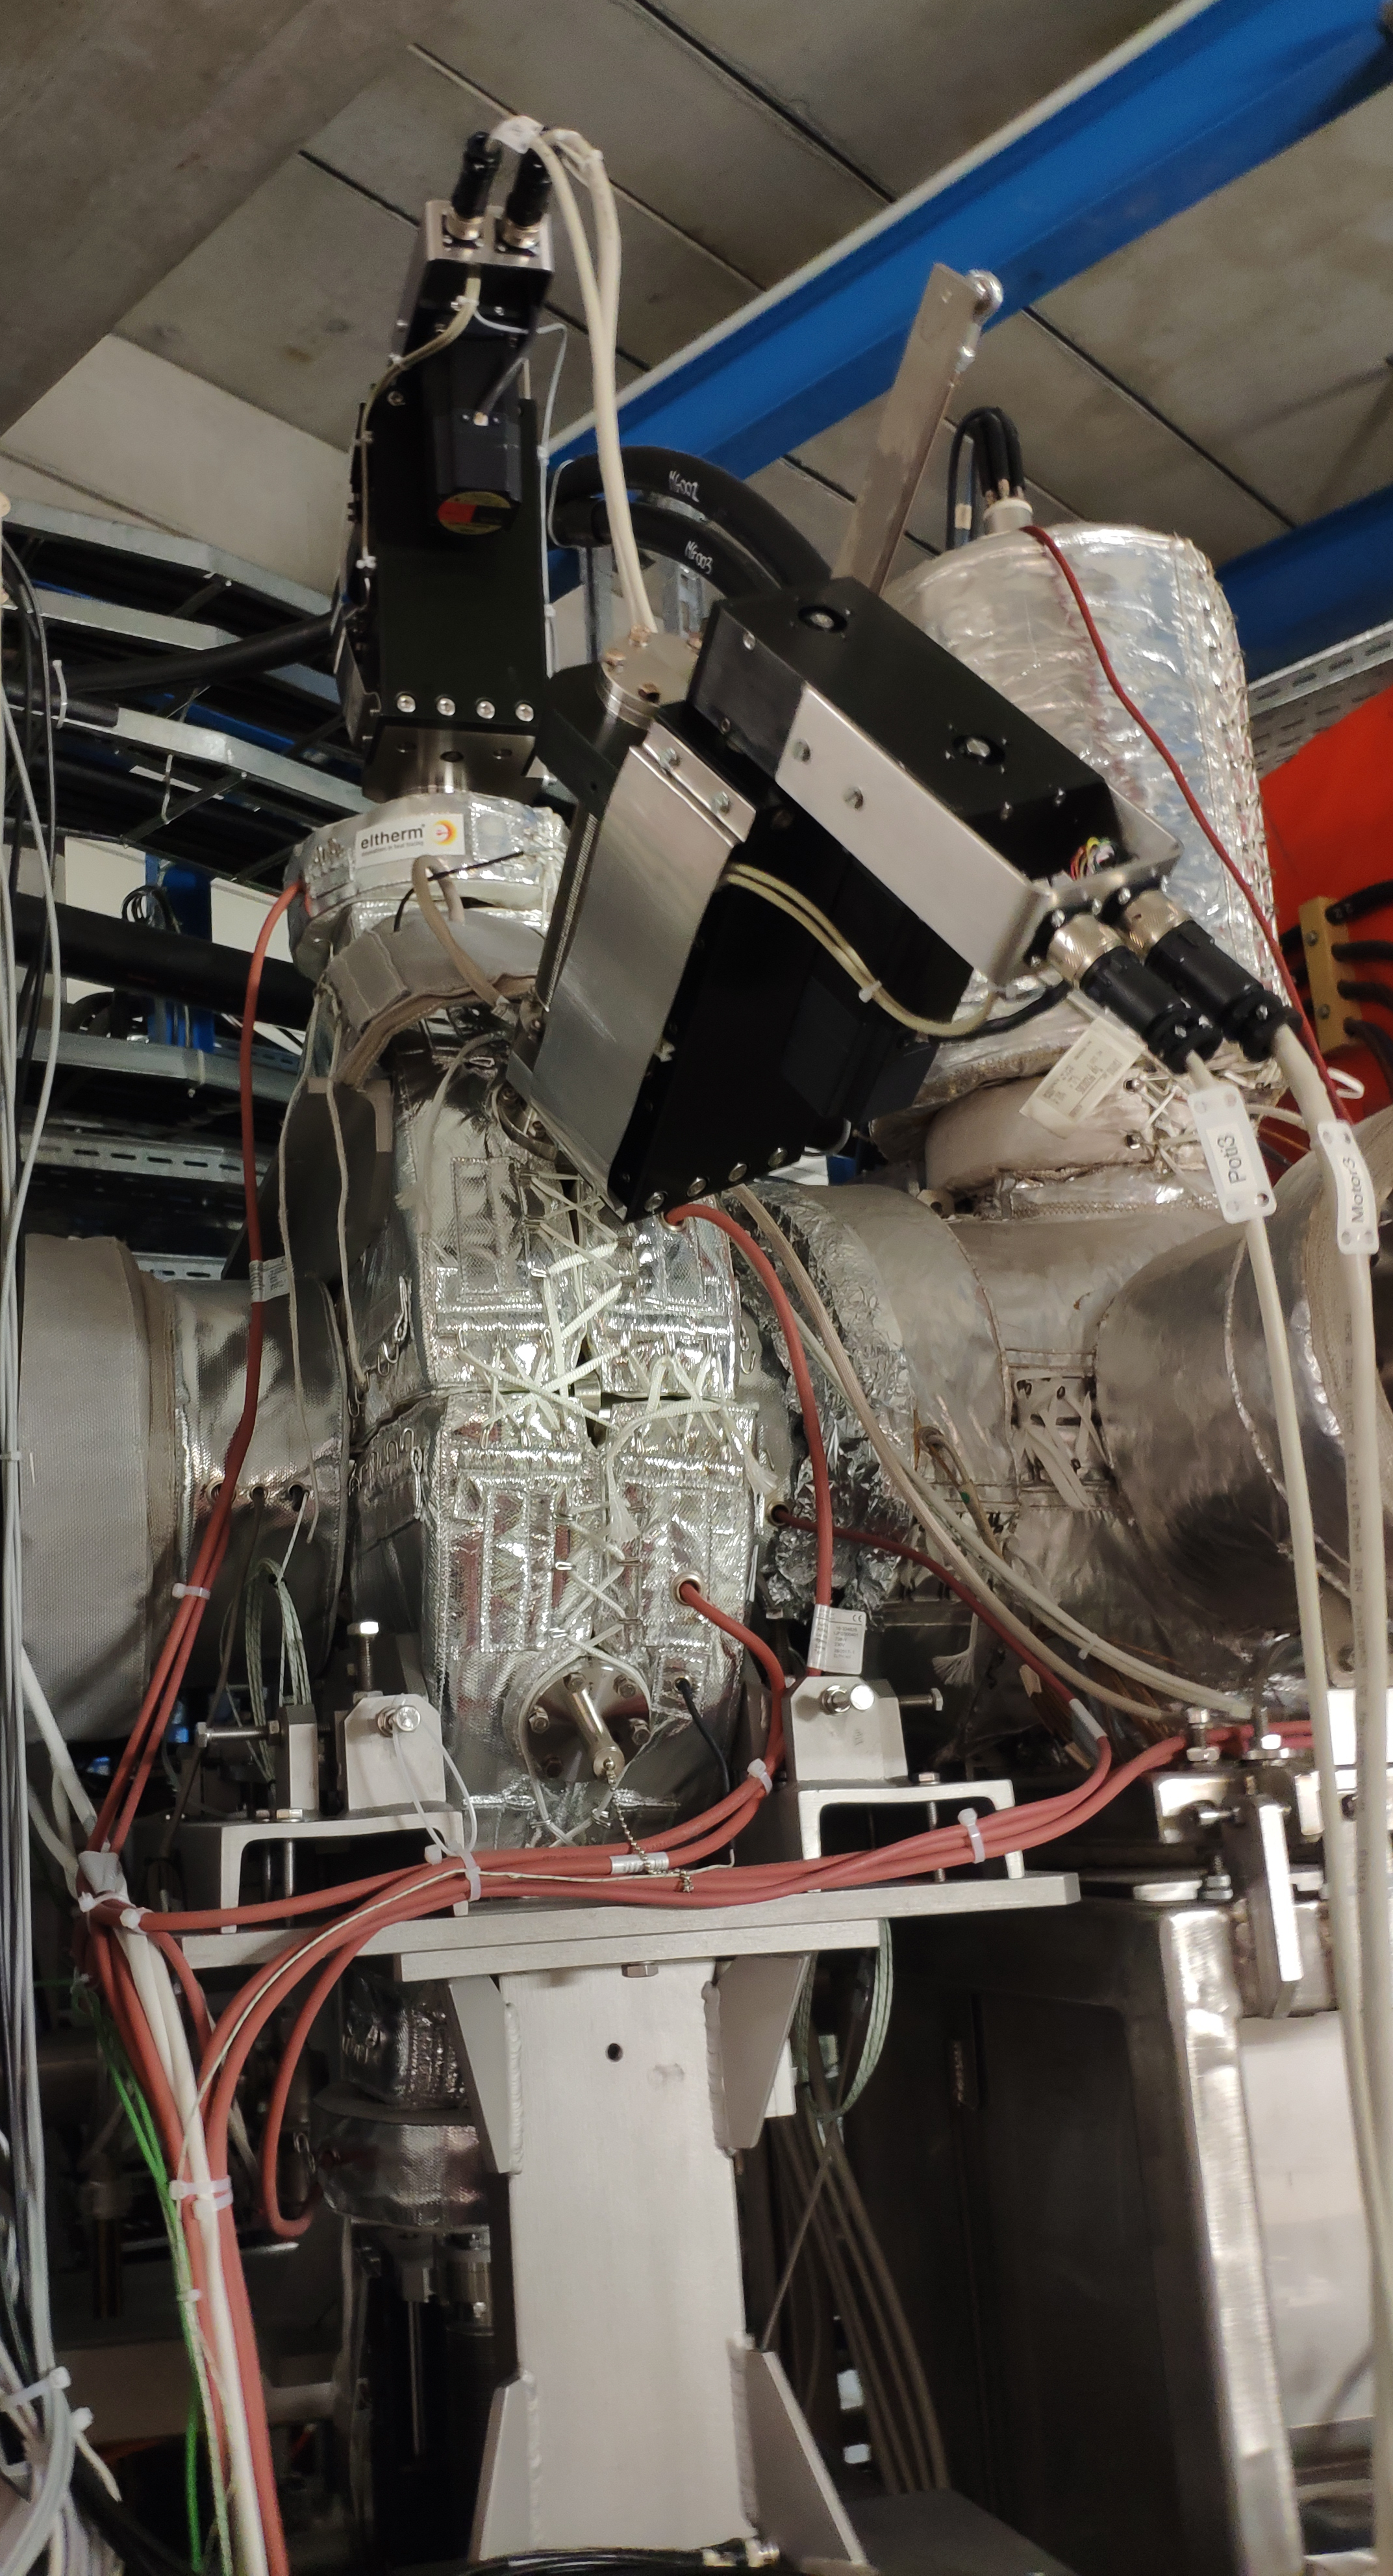
\includegraphics[width=0.25\textwidth]{410schottky.jpg}
        \label{fig:chap2:410}
    }
    \caption{Pictures of the Schottky cavities present at the \textsc{ESR}.}
    \label{fig:chap2:schottkies}
  \end{figure}
Charged particles traversing a beam pipe drag an opposite equivalent charge on its inner surface. In the surfaces of isolated sections, such as detector plates, this surface charge oscillates and dissipates \cite{schottky_book}, measurable as an induced current $i(t)$\footnote{It is important to note that the induced current itself is not directly measured. Instead, the voltage drop resulting from this current's interaction with the detector's impedance is recorded, which generally is frequency dependent.}.
A \textbf{similar} charge redistribution occurs on cavity walls, differing mainly in duration. This results in an oscillating electric dipole and an alternating magnetic field, with energy oscillations between both fields continuing after the particle passes through, as illustrated in \cref{fig:chap2:schottkysketch}. This oscillation is measured by extracting field energy with an electric pin or magnetic loop \cite{shahab_thesis,Sanjari_2013,Sanjari-410}.
\newpar
\begin{figure}[hbt]
    \centering
    \includegraphics[width=\textwidth]{schottky_sketch2.png}
    \caption{General sketch of a resonant Schottky cavity.}
    \label{fig:chap2:schottkysketch}
\end{figure}
For multiple particles, the induced current $i(t)$ becomes a stochastic process due to the random phase offsets\footnote{Not all the particles reach the detectors at the same time, they are randomly distributed.} between particles. The expected value of this process equates to the macroscopic direct current (DC) beam current $I_B$, formulated as $\langle E [i(t)] \rangle = Qef_r N = I_B$~\cite{shahab_thesis}, where $N$ represents the number of particles, $e$ the elementary charge, $Q$ the charge state, and $f_r$ the revolution \textsc{eigenfrequency}. Spectral analysis reveals peaks at integer multiples, \textsc{harmonics}~($h$), of the \textsc{eigenfrequency}, known as \textsc{Schottky bands}. These bands present a decrease in peak amplitude and an increase in width with higher harmonics (as can be seen in \cref{fig:app2:harmonics}), suggesting a \textbf{constant} integral power across all bands \cite{schottky_book}. The total noise power is given by \cite{CaspersSchottky}:
\begin{equation}
    \langle I \rangle^2 = 2N\left(Qef_r\right)^2.
    \label{eq:chap2:schottkyI}
\end{equation}
These non-destructive cavity detectors exhibit impedance spectra with pronounced peaks at their \textsc{eigenfrequencies}. This characteristic is exploited to enhance detection sensitivity and resolution at higher frequencies, albeit at the expense of operating within a narrow bandwidth. In contrast, parallel plate detectors tend to display a simpler impedance spectrum, potentially offering a broader operational frequency range but with different sensitivity and resolution profiles \cite{shahab_thesis}. 
For having the best of both worlds, at the \textsc{ESR} we have two Schottky cavities and a parallel plate Schottky. Among the Schottky cavities, one works at $245$\,MHz of resonant frequency and the other has an operational resonance frequency at $410$\,MHz. In comparison to the $410$\,MHz detector, the $245$\,MHz cavity has a smaller quality factor, which translates into a poorer signal-to-noise ratio ($S/N$). Although both detectors are single-ion sensitive, the difference in $S/N$ means that the $245$\,MHz detector requires a longer detection time.

\mybox{blue!70!black}{\textbf{Can there be a resonant Schottky cavity (RSC) everywhere?}}{
    Apart from non-physical reasons, the answer is no. \textsc{RSCs} have a high quality factor, or in other words, a high impedance which is coupled to the rest of the circuits. Due to its high impedance, it can lead to destructive effects~\cite{Sanjari-410} on the beam for cases in which the intensity is high (in terms of number of particles) or really high velocities. Around $1$\,GeV/nucleon these effects could be observed.
  }
\subsubsection{Data acquisition}\label{subsubsec:chap2:dataacquisiton}
During the experiment, resonant Schottky cavities were employed for beam diagnostics and for measuring the revolution spectra. To this end, each Schottky was connected to a real-time spectrum analyzer (\textsc{RSA}) of \textsc{Tektronix}$^{\circledR}$. These analyzers were centered in time around the injections and recorded $5$\,seconds of data before and after this time. In addition, the $245$\,MHz Schottky was connected to a continuous time and broadband recording device, the \textsc{NTCAP}~\cite{NTCAPpaper, NTCAPphd}.
%RSA sampling frequency and nsamples
%NTCAP sampling frequency and nsamples
% States that NCAP contains files with 56 seconds of data, and continuously for hours STRESS IT.
\newpar
The \textsc{RSAs} are specially useful for the fast in-line monitoring of specific isotopes and their half-lives. However, for performing mass measurements and optimizing the setting we need a broader picture. This can be facilitated by the \textsc{NTCAP} system, which also enabled the concurrent recording of scalar signals, including kicker time, cooler voltage, cooler current, gas target pressure, \textsc{SIS} kicker signal, \textsc{ESR} \textsc{DCCT} current, gas target status, and the raw kicker signal.
Moreover, the \textsc{NTCAP} provides a higher time resolution of $50$\,ns compared  to the $\sim 20\,\mu$s offered by the \textsc{RSAs}. This allows more accurate determination of injection times, as is discussed in \cref{subsubsec:chap2:injectiontime}.

\section{Isochronous mode}\label{sec:chap2:isomode}
In this section, I address how the isochronous mode condition can be measured in-line (\cref{subsec:chap2:ecoolercurve}) and off-line (\cref{subsec:chap2:isocurve}).

\subsection{Electron cooler curve}\label{subsec:chap2:ecoolercurve}
As previously discussed in \cref{subsubsec:intro:isoMS}, the isochronous mode occurs when $\gamma \rightarrow \gamma_t$. This signifies that ions of the same species become isochronous with each other, reaching the detector at the same frequency (\textsc{isochronously}) regardless of their velocities. This peculiar feature can be found by performing an energy scan to identify an energy region where, despite increasing the ion's energy, their revolution frequency remains unchanged. 
\newpar
In storage rings, such an energy scan is feasible through electron cooling, as introduced in \cref{subsubsec:intro:ecooling}. \Cref{fig:chap2:ecurve2014} illustrates this scanning process, measured in $2014$\footnote{Unfortunately, during experiment \textsc{E143}, no $2$D spectrogram was recorded from the electron cooler curve. Since $2$D spectrograms clearly demonstrate the followed procedure, I have analyzed older data for explanatory purposes.} by Schottky cavity detectors, in both 2D (\cref{fig:chap2:ecurve2014_2d}) and 1D (\cref{fig:chap2:ecurve2014_1d}) spectra. In \cref{fig:chap2:ecurve2014_2d} each frequency shift\footnote{Every $5$ seconds.} over time indicates a change in the electron cooler's voltage\footnote{Corresponding to $50$\,eV per step.}, hence in its energy, which progressively increases. This leads to a decrease in revolution frequency until reaching a specific region where further energy increments do not affect the frequency. This zone is identified as the \textsc{isochronous window}. ``Surprisingly", beyond this point, as energy continues to rise, the frequency increases. This phenomenon occurs because, similar to earlier when energy augmentation led to increased velocity and consequently lower revolution frequency, post-transition, the increment in path length predominates over the velocity gain. Eventually, this results in orbits becoming unsustainable within the ring's acceptance, causing collisions with the ring walls hence losing the ions. Therefore, with this procedure we can obtain the ion-optical parameter $\gamma_t$. 
\begin{figure}[hbt]
    \centering
    \subfloat[Electron cooler curve spectrogram.]{
        \includegraphics[width=0.33\textwidth]{ecurve2014_2d2.png}
        \label{fig:chap2:ecurve2014_2d}
    }
    \hspace{0.1cm}
    \subfloat[Electron cooler curve spectrum.]{
        \includegraphics[width=0.6\textwidth]{ecurve2014_1d_text.png}
        \label{fig:chap2:ecurve2014_1d}
    }
    \caption{Electron cooler curve. Every $5$\,seconds the primary beam's energy is increased by $50$\,eV through the electron cooler.}
    \label{fig:chap2:ecurve2014}
  \end{figure}
\newpar
Despite being determined solely with one species (the primary beam), the parameter is independent of the ions, representing an intrinsic property of the ring. Consequently, this parameter remains constant provided the magnet configuration is not changed. The width of the \textsc{isochronous window} can be tuned using sextupole and octupole magnets. Ideally, within the \textsc{ESR} acceptance, the revolution frequency should be the same for all the allowed energies, resulting in peak spreads following a Dirac's delta. This scenario is theoretically possible as each ion would follow a unique path, hence eliminating the possibility of Coulomb or other interactions between the ions. Thus, \textsc{IMS} has the potential to achieve superior mass resolution compared to \textsc{SMS}. Nonetheless, the situation is not entirely straightforward; crossing the transition point~\cite{transitioncrossing} can induce resonances in the beam (as observed in \cref{fig:chap2:ecurve2014_2d}), complicating the analysis. This phenomenon needs more investigation.

\mybox{blue!70!black}{\textbf{Is Cooled Isochronous Mass Spectrometry (CIMS) feasible?}}{
    When we cool the ions by any means, all of them share the same velocity after a certain time. Due to this, as already described in \cref{subsec:intro:cooling}, it can occur intra-beam scattering due to the Coulomb repulsion between ions of the same species. Therefore, this sets a limit on how reduced the momentum spread can be to where the Coulomb repulsion and the cooling force are in equilibrium. However, in \textsc{IMS} the ions do not share the same orbit, so in principle this limit is removed and, theoretically speaking, the \textsc{IMS} could have more potential for mass spectrometry. Now, if we try to cool the \textsc{IMS}, by definition we are forcing the ions to follow some specific orbit, hence destroying the working principles of \textsc{IMS}. A different (and worth testing) approach would be: 
    \begin{enumerate}
        \item Inject the fragments into the \textsc{ESR}.
        \item Cool them.
        \item Turn off the cooling.
        \item Adjust $\gamma_t$ (if necessary).
    \end{enumerate}
    Incorporating cooling limits the half-life of the studied nuclides to $\gtrsim1$\,s.
  }
\subsection{Peak spread curve}\label{subsec:chap2:isocurve}

Ultimately, the \textsc{isochronicity} is also manifested in the measurable time (frequency) spread of peaks, denoted as $\sigma_t$. In such a way, through offline analysis is possible to deduce the transition energy parameter ($\gamma_t$) among other beam parameters, such as the relative momentum spread ($\sigma_p/p$) and the systematic errors ($\sigma_{sys}$), as contained in the equation (refer to \cref{apdx:derivations} for its derivation):
\begin{equation}\label{eq:chap2:sigma_T_final}
    \sigma_T = \sqrt{\left(\left(1 - \left(\frac{L}{T \cdot c }\right)^2 - \frac{1}{\gamma_t^2}\right)\cdot\left(\frac{\sigma_p}{p}\right)\cdot T\right)^2 + \sigma_{sys}^2},
\end{equation}
where $L$ represents the particle path length, and $c$ is the speed of light in vacuum. By applying a fitting procedure, we can estimate the average values of these parameters.
\newpar
The impact of varying the parameters in \cref{eq:chap2:sigma_T_final} offers valuable insights into the behavior and implications of the resulting curves. Examining the effects of adjusting one parameter while fixing the others constant reveals:
\begin{itemize}
    \item Modifying the ring's transition energy shifts the isochronicity curve to different $m/q$ regions. The effect would be similar to modifying the Lorentz factors ($\gamma$) of isotopes while keeping $\gamma_t$ fixed, as the curve's minimum corresponds to a specific energy/revolution time in the ring. Adjusting the settings of the storage ring can result in unpredictable behavior of the beams stored in the \textsc{ESR}. Therefore, modifying the gamma values presents a more practical and manageable approach, since the ion-optical setting will remain fixed and well-characterized. Furthermore, when employing Schottky resonant cavities, there is no need to alter neither their resonant frequency once fixed in the frequency corresponding to $\gamma_t$. Although, adjustments to the resonant frequency can be made by slightly modifying the cavity dimensions.

    \item Altering the particles' relative momentum spread can enhance the overall mass resolving power by flattening the \textsc{isochronicity curve}, albeit without improving the peak resolution within the isochronicity window, this is the minima will not be lower as can be seen in \cref{fig:chap2:isocurve-dp_p}.

    \item The maximum\footnote{How far from $0$ is the minimum peak width.} achievable resolving power is constrained by unidentified sources of uncertainty. It comes from second order terms in \cref{eq:intro:basic} mainly related to the magnet settings.

\end{itemize}

\mybox{blue!40!black}{\textbf{How does changing the Lorentz factor affect the isochronicity curve?}}{
    Since this term solely depends on the longitudinal velocity of the ions, producing ions with slightly higher (lower) velocities results in a shift of the entire frequency pattern towards lower (higher) frequencies. Consequently, its effect might be camouflaged as a (broader) standard deviation, especially when considering the overlay of different injections under the same magnetic settings. The velocity of the generated fragments is primarily influenced by the energy obtained by the primary beam during the acceleration stage, which can vary slightly from one injection to another. Hence, frequency correction (refer to \cref{subsubsec:chap2:freqcorrection}) is essential for removing this additional uncertainty and improving the measurement accuracies.
}

\begin{figure}[hbt]
    \centering
    \subfloat[Variations of the transition energy ($\gamma_t$).]{
    \includegraphics[width=0.48\textwidth]{isocurve-gammat.png}
    \label{fig:chap2:isocurve-gammat}
    }
    \vspace{0.5cm}
    \subfloat[Variations of the relative momentum spread ($\sigma_p/p$).]{
    \includegraphics[width=0.48\textwidth]{isocurve-dp_p.png}
    \label{fig:chap2:isocurve-dp_p}
    }
    \vspace{0.5cm}
    \subfloat[Variations of the systematic uncertainties ($\sigma_{sys}$).]{
    \includegraphics[width=0.48\textwidth]{isocurve-systematics.png}
    \label{fig:chap2:isocurve-systematics}
    }
    \caption{Change of behaviors of the isochronicity curve by considering each parameter in \cref{eq:chap2:sigma_T_final} independent.}
    \label{fig:chap2:iso_parameters}
  \end{figure}

%With the kicker the ions are injected in the outside orbits of the acceptance of \textsc{ESR}, covering a $30$~\% of the outer orbits of \textsc{ESR} acceptance. With cooling, we can change from outer orbits to internal orbits. This is necessary to perform a bunching of the beam.

\section{Data manipulation}\label{sec:chap2:datamanipulation}
In this section, I outline the process for selecting high-resolution data from a total dataset of $46$\,TB (\cref{subsec:chap2:dataclassification}), and how it was processed for performing mass (\cref{subsec:chap2:massdetermination}) and half-life (\cref{subsec:chap2:halflifedetermination}) measurements.
\subsection{Data classification}\label{subsec:chap2:dataclassification}
Here, I describe how the high-resolution data was recorded (\cref{subsubsec:chap2:recorded}), selected (\cref{subsubsec:chap2:exploratory}) and pre-processed (see \cref{subsubsec:chap2:injectiontime} and \cref{subsubsec:chap2:freqcorrection}).
\subsubsection{Recorded data}\label{subsubsec:chap2:recorded}

The process of converting ion-induced periodic signals into a measurable form involves transforming these signals into voltage drops across a circuit, captured within a finite temporal resolution. Therefore, since the moment we record the data we are losing information. Subsequent stages involve the refinement and simplification of this physical information through various amplification and mixing circuits, culminating in the digital storage of data in binary format. To facilitate data access and manipulation of Schottky-based data, the \textsc{iqtools}~\cite{iqtools} \textsc{Python} library was developed.
\subsubsection{Exploratory data analysis}\label{subsubsec:chap2:exploratory}

The initial phase of data analysis focuses on differentiating between usable and non-usable data. With the help of the experimental electronic log, which can be found in \cite{e143elog}, we can check when there was a stable\footnote{Without any operational issues.} beam or not, and verify them through preliminary analysis. In this way, we can constrain significantly the data to analyze. Subsequently, we explore ``macroscopic" features, such as the signal-to-noise ratio, total power across the bandwidth and count, location, and shape of peaks. Data injections sharing similar characteristics are then classified into the same subset. Within these data subsets, the injection times are identified, and optimal \textsc{FFT} parameters for our analysis needs are determined.
\subsubsection{Determination of the injection time}\label{subsubsec:chap2:injectiontime}
While injection times are clearly marked in \textsc{RSA} data, this is not the case for \textsc{NTCAP} data. Given the voluminous data, locating them is challenging. To accurately identify injection times in the continuous \textsc{NTCAP} data, I searched for features of injection, such as frequency shifts and power fluctuations over time, utilizing the latter for its robustness and superior time resolution, which utilizes the data's maximum temporal resolution ($\sim$\,nanoseconds for the \textsc{NTCAP} data, see \cref{subsubsec:chap2:dataacquisiton}). For this purpose, I developed the software \textsc{TDMchopS} \cite{freire_fernandez_2023_8172227}.
\newpar
\begin{figure}[hbt]
    \centering
    \subfloat[Power fluctuations around injections.]{
        \includegraphics[width=0.75\textwidth]{injection_fluctuation.png}
        \label{fig:chap2:injection_fluctuation}
    }
    \vspace{0.1cm}
    \subfloat[Moving average of $30$\,ms.]{
        \includegraphics[width=0.75\textwidth]{injection_fluctuation_mave.png}
        \label{fig:chap2:injection_fluctuation_mave}
    }
    \caption{Power fluctuations around injections serve as a reliable indicator for determining injection times with the highest precision given by the sampling time.}
    \label{fig:chap2:injection_fluctuations}
\end{figure}

This technique has been named the \textsc{V-method}, reflecting the shape of the moving average as depicted in \cref{fig:chap2:injection_fluctuation_mave}. It is based on the empirical observation that approximately $30$\,ms before a new injection, the preceding signal within the \textsc{ESR} almost completely disappears (see \cref{fig:chap2:injection_fluctuation}), indicated by a sudden decrease in total recorded power, and therefore in the number of ions stored. To precisely identify the moment of injection, we apply a moving average over a span of $30$\,ms, where the minimum reveals the exact injection time, resulting in a distinctive \textsc{V-shape}.
\newpar
The underlying reasons for this intensity fluctuations are not fully understood and require of further investigations. It is believed that residual magnetic fields in the kicker magnet could lead to this characteristic phenomenon.

\subsubsection{Frequency correction and add-up}\label{subsubsec:chap2:freqcorrection}
After defining our data subsets, processing them through \textsc{FFT}, and finding the injection time, we aggregate all spectra together. This approach allows us to retain the entirety of the physical information while significantly reducing the data volume for subsequent analysis, from $\sim$\,Terabytes to $\sim$\,Gigabytes.
\newpar
Firstly, we add all the spectra without taking any reference peak. This is termed \textsc{blind sum}.
Next, we select one of the peaks with the highest yield\footnote{Since it will be present (ideally) in all the injections, so the reference will not change.}, and we use it as a reference peak to center individually each spectrogram to the same reference frequency. This step, although altering the frequency information, corrects for magnetic instabilities (via \textsc{software cooling}) and for fluctuations in $\gamma$ values across different injections as well as within single injections, hence enhancing data quality while maintaining all the information.
%One might question the legitimacy of this process: Does aligning spectrograms to a common frequency alter the physical information they contain? 

\subsection{Schottky-based ion identification}\label{subsec:chap2:identification}
After pre-processing, we can proceed with the identification of \textbf{every} peak and the determination of its characteristic: location, spread and shape. For this, we rely on the developed python library \textsc{RionID}~\cite{rionid} (Ringed ion IDentification) and Gaussian fitting.
\subsubsection{\textsc{RionID}}\label{subsubsec:chap2:rionid}

The \textsc{RionID}~\cite{rionid} software plays a key role in peak identification, based on overlaying simulated (ideal) ion revolution frequencies onto the experimental data. Deviations between the simulated and real data are observed, as expected due to the influence of the velocity spread term in \cref{eq:intro:basic}. These deviations typically follow a parabolic behavior as have been empirically observed. Therefore, they can be corrected, extending the correctness of the simulation to the whole measured frequency range.
\newpar
To emphasize that in \cref{eq:intro:basic} we are relating the ``distances'' of various parameters relative to a reference particle, we introduce the subscript $_i$ for each ion, and $_r$ for the reference ion, resulting in:
\begin{equation} 
    \frac{{\Delta}f_{i}}{f_{r}} = -\frac{1}{\gamma_{t}^{2}}\frac{{\Delta}\left(\frac{m}{q}\right)_{i}}{\left(\frac{m}{q}\right)_{r}}+\left(1-\frac{\gamma_{i}^{2}}{\gamma_{t}^{2}}\right)\frac{\left(\Delta v\right)_{i}}{v_{r}}.
    \label{eq:chap2:basis_i} 
\end{equation}
To simplify our simulation of expected revolution frequencies, we adopt a first-order \textbf{approximation} by neglecting the second term in \cref{eq:chap2:basis_i}. Therefore, the resulting formula for the simulated revolution frequency of an ion $i$ is:
  \begin{equation}
    f^{\mathrm{s}}_{i} =f_{r} \cdot\left(1-\frac{1}{\gamma_{t}^{2}}\frac{{\Delta}\left(\frac{m}{q}\right)_{i}}{\left(\frac{m}{q}\right)_{r}}\right),
    \label{eq:chap2:basis_i2}
  \end{equation}
where we assume the same $\gamma_t$ for every ion.
\newpar
As expected, empirically we observe that the simulated $f^{\mathrm{s}}_{i}$ do not match the experimentally measured frequencies for many ions (specially the ones outside the isochronous window). Investigating the difference between experimental and simulated (superscripts $^\mathrm{e}$ and $^\mathrm{s}$, respectively) revolution frequencies $f^{\mathrm{e}}_{i}$ - $f^{\mathrm{s}}_{i}$ reveals a parabolic dependence with frequency (as can be seen in \cref{fig:chap2:deviationsRionID}), expressed as:
\begin{equation} 
    f^{\mathrm{e}}_{i} - f^{\mathrm{s}}_{i} = a + b\cdot f^{\mathrm{s}}_{i} + c \cdot \left(f^{\mathrm{s}}_{i}\right)^2.
    \label{eq:chap2:basis_i3} 
\end{equation}

\begin{figure}[hbt]
    \centering
    \subfloat[Data of May $2021$ from \textsc{E143}.]{
        \includegraphics[width=0.47\textwidth]{correct_identification72Ge.png}
        \label{fig:chap2:ident_correction1}
    }
    \hspace{0.05cm}
    \subfloat[Data of June $2021$ from \textsc{E143}.]{
        \includegraphics[width=0.47\textwidth]{correct_identification70Se_june.png}
        \label{fig:chap2:ident_correction2}
    }
    \caption{Comparison between simulated and measured frequencies, alongside the fit and its residuals for two different data subsets.}
    \label{fig:chap2:deviationsRionID}
\end{figure}

This implies:
\begin{equation} 
    f_{r} \cdot\left(1-\frac{\gamma_{i}^{2}}{\gamma_{t}^{2}}\right)\frac{\left(\Delta v\right)_{i}} {v_{r}} = a + b\cdot f^{\mathrm{s}}_{i} + c \cdot \left(f^{\mathrm{s}}_{i}\right)^2,
    \label{eq:chap2:basis_i5} 
    \end{equation}

because, by definition (combining \cref{eq:intro:basic} and \cref{eq:chap2:basis_i2}):
\begin{equation} 
    f^{\mathrm{e}}_{i} = f^{\mathrm{s}}_{i} + f_{r} \cdot\left(1-\frac{\gamma_{i}^{2}}{\gamma_{t}^{2}}\right)\frac{\left(\Delta v\right)_{i}}{v_{r}}.
    \label{eq:chap2:basis_i4} 
\end{equation}
Hence, the velocity information is encapsulated within the polynomial fitting.
\newpar
Identifying particles within the \textsc{isochronous window} becomes straightforward since the approximation \cref{eq:chap2:basis_i2} is valid enough, although we can already notice a small parabolic deviation.  By fitting this deviation with \cref{eq:chap2:basis_i3}, we can obtain the polynomial coefficients and correct the deviation. After making these corrections, there is nearly a direct match between the simulated and observed peaks within the whole spectrum, as illustrated in \cref{fig:chap2:deviationsRionID}. However, the potential for erroneous identifications exists due to the overlap of harmonics and the large amount of possible fragments. This is explored in \cref{subsubsec:chap2:harmonicoverlapping}.

\subsubsection{Harmonic overlapping}\label{subsubsec:chap2:harmonicoverlapping}
Non-destructive Schottky cavity detectors enhance beam monitoring and facilitate precise mass and half-life measurements, as highlighted in \cref{subsubsec:chap2:schottkyCR}.
Pursuing higher mass (frequency) resolution requires higher resonant frequencies, or equivalently, higher harmonics. However since the Schottky bandwidth increases linearly with the harmonic number, we encounter the issue of \textsc{harmonic overlap}. This phenomenon causes different ion species at distinct harmonics to coincide at the same revolution frequency, potentially leading to signal contamination. Therefore, we need to develop different identification strategies to identify and solve this contamination.
The most recent Schottky cavities~\cite{Sanjari_2013,Sanjari-410} typically operate within the $(120,130)$ and $(208,215)$ harmonic ranges, where between $(8,16)$ harmonic superpositions may occur within the same measured frequency spectrum, as demonstrated in \cref{fig:chap2:overlaps}.
\begin{figure}[hbt]
    \centering
    \includegraphics[width=0.70\textwidth]{count_overlaps.png}
    \caption{%
        Number of overlaps as a function of the harmonic number, assuming an infinite number of Schottky bands. $f_c$ and $f_s$ denote the average \textsc{eigenfrequency} and \textsc{bandwidth}, as measured in a data subset of experiment \textsc{E143}, respectively.
    }\label{fig:chap2:overlaps}
\end{figure}
A mathematical investigation into harmonic overlap is addressed in \cref{apdx:harmonicoverlap}.
\newpar
To unambiguously identify each species, several strategies can be utilized:
\begin{itemize}
    \item Verify the presence of the same peak across different harmonics, since each species has a unique \textsc{eigenfrequency}.
    \item Examine the shape and spread of neighboring peaks for consistency, since they should be similar to other ions in the same mass-to-charge region.
    \item Perform a mass measurement to check for significant deviations from the expected values, indicating potential misidentification.
\end{itemize}
These procedures help to confirm the identification of each peak and whether it has contamination. The subsequent challenge is determining how to effectively use data that may be contaminated.
A potential solution to the contamination lies in peak deconvolution, aiming to isolate the true peak from overlapping signals. This approach, however, demands precise knowledge of the peak shape at the given revolution frequency, which is complex to model. More information can be found in \cref{apdx:peakshapedeconvolv}.
\newpar
Once we have identified our ions, we determine the mean and standard deviations of the peak distributions by means of Gaussian fitting, and we feed this values to the mass (\cref{subsec:chap2:massdetermination}) and half-life (\cref{subsec:chap2:halflifedetermination}) determination routines.

\subsection{Mass determination}\label{subsec:chap2:massdetermination}

The detailed mathematical foundations of the commonly employed method for mass measurements at storage rings can be found in the precursor \cite{AUDIcmm}, other theses~\cite{YuriPhD,MatosPhD,ShubinaPhD}, and papers~\cite{RADONcmmA}. In this subsection, I will resume the concepts and how they were implemented in the \textsc{Python} library \textsc{RionMass}~\cite{rionmass} for performing mass measurements of summed-up isochronous spectra.
\newpar
Firstly, we import the experimental data: measured revolution frequency, harmonic number, ion species, peak width and their corresponding errors, and the Atomic Mass Evaluation~\cite{AME-2020} (\textsc{AME}) data for these ions (if known) and their electron binding energies~\cite{NIST_ASD}. For the \textsc{AME} data, we use the \textsc{Python} package \textsc{Barion}~\cite{barion} which already implements a connection to the \textsc{NUBASE}~\cite{Nubase2020} database and downloads the file, reads it and subtract information. For the electron binding energies, we scrap the data from ~\cite{NIST_ASD}. Once we have all the information, we pass to perform the calculations. 
\newpar
First, we perform a $P^\mathrm{th}$ order polynomial fit of the $m/q$ as a function of the revolution frequency (or time) of the reference ions. Consequently, we perform what is known as self-calibration. For every ion that we consider as a reference, we perform a \textsc{least-squares} fit of the (\textsc{AME}) mass-to-charge ratios as a function of the revolution frequency (time) with a $P^\mathrm{th}$ order polynomial iteratively trying to minimize our objective function, which is in this case a reduced chi-square ($\chi^2$): 
\begin{align} 
    &\left(\frac{m}{q}\right)_{i} = \sum_{p=0}^{P} a_{p}f_{i}^{p}, \label{eq:chap2:cmm1}\\
    &\left(\frac{m}{q}\right)_{r} = \left(\frac{m}{q}\right)_{\mathrm{AME2020}}, \label{eq:chap2:cmm1ame}\\
    &d \left(\frac{m}{q}\right)_{i} = \diff{\left(\sum_{p=0}^{P} a_{p}f_{i}^{p}\right)}{f_{i}} \sigma_{f_{i}}= \sum_{p=1}^{P} pa_{p}f_{i}^{p-1}\sigma_{f_{i}},\label{eq:chap2:cmm2}\\
    &\Delta \left(\frac{m}{q}\right)_{r} = \Delta \left(\frac{m}{q}\right)_{\mathrm{AME2020}}, \label{eq:chap2:cmm2ame}\\
    &\left(\frac{m}{q}\right)_{i} - \sum_{p=0}^{P} a_{p}f_{i}^{p} = l_{i} \pm \Delta_{i}, \label{eq:chap2:cmm3}\\
    &\chi^2 = min\left(\sum_{i=1}^{N}  \frac{\left(\left(\frac{m}{q}\right)_{i} - \sum_{p=0}^{P} a_{p}f_{i}^{p}\right)^2}{\left(\Delta \left(\frac{m}{q}\right)_{i,\mathrm{AME2020}}\right)^2 + \left(\sum_{p=1}^{P} pa_{p}f_{i}^{p-1}\sigma_{f_{i}}\right)^2}\right).\label{eq:chap2:chi2} 
\end{align}
This procedure is repeated for each reference ion ($N$ in total) by turning them ``off" as references, thus deriving their mass-to-charge ratio ($m/q$) from the fitting process while treating the $m/q$ ratios of all other reference ions as known, based on the \textsc{AME} values.
As a result, we acquire global fitting parameters~$a_p$ that minimize \cref{eq:chap2:chi2}. For any ions whose values are not previously known, their $m/q$ ratios can be determined using \cref{eq:chap2:cmm1}. 
\newpar
For high-precision mass measurements, we have to exclude reference ions with poor signal-to-noise ratio ($S/N$) and significant mass uncertainties (usually over $20$\,keV). This can be solved by establishing a criteria based on the amplitude under the peaks.
Moreover, it is essential to eliminate from our routine the peaks containing unresolved isomers, unresolved different ion species, contaminating signals from other harmonics, or noise. All of these contaminants are typically identifiable on the isochronicity curve \cref{subsec:chap2:isocurve} or, ultimately, at the mass measurement procedure.

\subsubsection{Excitation energy determination}\label{subsubsec:chap2:excitationenergydeter}
Mass measurements in storage rings are typically conducted using polynomial fitting, as described in \cref{subsec:chap2:massdetermination}. This method uses the information of all ions within the ring by using \cref{eq:intro:basic}. But, is it necessary or even optimal to use all of this information?
\newpar
I propose a simplified and intuitive approach applicable to the measurement of excitation energies. Assuming almost identical velocity distribution\footnote{Intuitively, considering the production mechanism, we can assume that both ground and isomeric states are produced with the same energy, but due to the isomer being excited, having less velocity.} between isomer and ground state, and that both are within the \textsc{isochronous window}, the second term of \cref{eq:intro:basic} is negligible. Moreover, taking into consideration that $\Delta m = w$ between the isomer and ground state, the expression is simplified to: 
\begin{equation}
    \omega=\frac{\Delta f}{f_{gs}}m_{gs}\gamma_t^2.
    \label{eq:chap2:isomer_energy} 
\end{equation}
The relative frequency distance ($\Delta f$) is calculated by determining the centroids and standard deviations of both distributions by, generally, Gaussian fitting. Finally, $\gamma_t$ can be determined from the isochronicity curve. Like this, we are using the information of all the ions but without introducing their mass errors into our measurements, which can constrain the precision on the isomer mass determined.

\subsection{Half-life determination}\label{subsec:chap2:halflifedetermination}
In this thesis, a \textbf{new approach} to determine the half-life of exotic\footnote{With low yield.} short-lived species has been developed. Unlike previous experiments, which continuously monitor beam loss post-injection~\cite{Litvinov-2003,PhysRevLett.99.262501,Litvinov-2008a} or counting frequency shifts~\cite{2013638,fatma}, our approach adds-up time-resolved spectra (as discussed in \cref{subsubsec:chap2:freqcorrection}) from multiple injections and does not directly count decaying particles; instead, we observe the signal's disappearance induced by these particles at specific frequency channels. This method differs fundamentally from that of ``traditional" particle detectors, like double-sided silicon strip detectors, which \textbf{physically intercept} reaction products.
\begin{figure}[hbt]
    \centering
    \includegraphics[width=0.6\textwidth]{isomeric_ratio_response.png}
    \caption{Linear relation between the mean number of ions and strength of the fluctuations in number of ions.}
    \label{fig:chap2:fluctuations}
\end{figure}
\newpar
Each injection may carry one or a few ions of interest, and the aggregate spectrum exhibits the characteristic decay curve, synchronized by the common injection time. 
It is important to stress that with \textsc{RSCs} we are single-ion sensitive when we have a few ions \cref{fig:chap2:fluctuations}. Therefore, this motivates us to do measurements with as few ions as possible and as many times (injections) as possible in order to exploit the single-ion sensitivity, which implies the adding-up technique.
\newpar
In such a way, when peaks are completely resolved, the measurement is straightforward: we have to select the frequency channels that contain the ion species and monitor their temporal evolution. For contaminated peaks, measurements can be conducted using the method outlined in \cref{apdx:peakshapedeconvolv}.
The integrated noise power of every peak in the summed spectrum is then directly proportional to the corresponding number of stored particles (as given by \cref{eq:chap2:schottkyI}).
The validity of this analysis approach has been thoroughly tested by dedicated \textsc{Monte Carlo} simulations \cite{mcshahab} and cross-checked by extracting individual decay times, the details of which will be published elsewhere.
\begin{center}
    \vspace*{1cm}
    \pgfornament[width=0.8cm, color=darkred]{5}
    %\pgfornament[width=5cm, color=darkred]{71}
    %\pgfornament[width=5cm, color=darkred]{71}
    \vspace*{\fill}
\end{center}